\documentclass{article}\usepackage[]{graphicx}\usepackage[]{color}
%% maxwidth is the original width if it is less than linewidth
%% otherwise use linewidth (to make sure the graphics do not exceed the margin)
\makeatletter
\def\maxwidth{ %
  \ifdim\Gin@nat@width>\linewidth
    \linewidth
  \else
    \Gin@nat@width
  \fi
}
\makeatother

\definecolor{fgcolor}{rgb}{0.345, 0.345, 0.345}
\newcommand{\hlnum}[1]{\textcolor[rgb]{0.686,0.059,0.569}{#1}}%
\newcommand{\hlstr}[1]{\textcolor[rgb]{0.192,0.494,0.8}{#1}}%
\newcommand{\hlcom}[1]{\textcolor[rgb]{0.678,0.584,0.686}{\textit{#1}}}%
\newcommand{\hlopt}[1]{\textcolor[rgb]{0,0,0}{#1}}%
\newcommand{\hlstd}[1]{\textcolor[rgb]{0.345,0.345,0.345}{#1}}%
\newcommand{\hlkwa}[1]{\textcolor[rgb]{0.161,0.373,0.58}{\textbf{#1}}}%
\newcommand{\hlkwb}[1]{\textcolor[rgb]{0.69,0.353,0.396}{#1}}%
\newcommand{\hlkwc}[1]{\textcolor[rgb]{0.333,0.667,0.333}{#1}}%
\newcommand{\hlkwd}[1]{\textcolor[rgb]{0.737,0.353,0.396}{\textbf{#1}}}%
\let\hlipl\hlkwb

\usepackage{framed}
\makeatletter
\newenvironment{kframe}{%
 \def\at@end@of@kframe{}%
 \ifinner\ifhmode%
  \def\at@end@of@kframe{\end{minipage}}%
  \begin{minipage}{\columnwidth}%
 \fi\fi%
 \def\FrameCommand##1{\hskip\@totalleftmargin \hskip-\fboxsep
 \colorbox{shadecolor}{##1}\hskip-\fboxsep
     % There is no \\@totalrightmargin, so:
     \hskip-\linewidth \hskip-\@totalleftmargin \hskip\columnwidth}%
 \MakeFramed {\advance\hsize-\width
   \@totalleftmargin\z@ \linewidth\hsize
   \@setminipage}}%
 {\par\unskip\endMakeFramed%
 \at@end@of@kframe}
\makeatother

\definecolor{shadecolor}{rgb}{.97, .97, .97}
\definecolor{messagecolor}{rgb}{0, 0, 0}
\definecolor{warningcolor}{rgb}{1, 0, 1}
\definecolor{errorcolor}{rgb}{1, 0, 0}
\newenvironment{knitrout}{}{} % an empty environment to be redefined in TeX

\usepackage{alltt}
\usepackage{natbib}
\usepackage[unicode=true]{hyperref}
\usepackage{geometry}
\geometry{tmargin=1in,bmargin=1in,lmargin=1in,rmargin=1in}


\IfFileExists{upquote.sty}{\usepackage{upquote}}{}
\begin{document} 
\title{STAT243-PS5}
\author{Jinhui Xu}
\date{October 2017}

\maketitle

\section{Other students}
I discuss some problems with Weijie Xu
\section{Question 2}

\subsection{(a)}
First, we look at the format $(-1)^S*1.d*2^{e-1023}$. 
As d is represented as 52 bits and e is represented as 11 bits, we can write the format as  $$(-1)^S*1.d_{1}d_{2}...d_{52}*2^{e-1023}=(-1)^S*(1+d_{1}*2^{-1}+d_{2}*2^{-2}...+d_{52}*2^{-52})*2^{e-1023}$$ where $S,d_{i} \in \{0,1\}$ and $(e-1023) \in \{-1023,-1022,...,1024,1025\}$\\

Then let $2^p-m$ is any one number among $\{1,2,3,...,2^{53}-2,2^{53}-1\}$ where $m \in \{1,2,...,2^p-1\}$. Obviously, S=0 and we can find a group of $d_{i}$ that makes $$(1+d_{1}*2^{-1}+d_{2}*2^{-2}...+d_{52}*2^{-52})*2^{p-1}=2^p-m$$ It is because the range of the left of the equation is $[2^{p-1},2^{p}-2^{p-53}]$ and the precision is $2^{p-53}$\\

For example\\
$$2^{53}-2=(1+1*2^{-1}+,...,+1*2^{-50}+1*2^{-51}+0*2^{-52})*2^{52},which\ means\ d_{52}=0\ and\ other\ d_{i}=1$$
$$2^{52}-3=(1+1*2^{-1}+,...,+0*2^{-50}+1*2^{-51}+0*2^{-52})*2^{51},which\ means\ d_{50,52}=0\ and\ other\ d_{i}=1$$

\subsection{(b)}
If we want to store $2^{53},2^{53}+1,2^{53}+2,...$, from $(a)$, we can know that p=54. In this way, the precision equals to $2^{p-53}=2$\\
It is the same situation when we store $2^{54},2^{54}+1,2^{54}+2,...$. In this situation, p=55. Then the precision equals to $2^{p-53}=4$
\begin{knitrout}
\definecolor{shadecolor}{rgb}{0.969, 0.969, 0.969}\color{fgcolor}\begin{kframe}
\begin{alltt}
\hlkwd{options}\hlstd{(}\hlkwc{digits}\hlstd{=}\hlnum{22}\hlstd{)}
\hlkwd{print}\hlstd{(}\hlnum{2}\hlopt{^}\hlnum{53}\hlopt{-}\hlnum{1}\hlstd{)}
\end{alltt}
\begin{verbatim}
## [1] 9007199254740991
\end{verbatim}
\begin{alltt}
\hlkwd{print}\hlstd{(}\hlnum{2}\hlopt{^}\hlnum{53}\hlstd{)}
\end{alltt}
\begin{verbatim}
## [1] 9007199254740992
\end{verbatim}
\begin{alltt}
\hlkwd{print}\hlstd{(}\hlnum{2}\hlopt{^}\hlnum{53}\hlopt{+}\hlnum{1}\hlstd{)}
\end{alltt}
\begin{verbatim}
## [1] 9007199254740992
\end{verbatim}
\end{kframe}
\end{knitrout}
We can find that $2^{53}+1$ is stored same as $2^{53}$ in R. Because the precision is 2.

\section{Question 3}
\subsection{(a)}
Copy two vectors and it is obviously that copying numeric vector takes more time. It is because that storing each int in R takes 4 bytes while storing each numeric in R takes 8 bytes. In plot, I use log function to the data.
\begin{knitrout}
\definecolor{shadecolor}{rgb}{0.969, 0.969, 0.969}\color{fgcolor}\begin{kframe}
\begin{alltt}
\hlkwd{library}\hlstd{(data.table)}
\hlkwd{library}\hlstd{(microbenchmark)}

\hlcom{#the function to compare the time used to copy two item.}
\hlstd{compare_copytime}\hlkwb{=}\hlkwa{function}\hlstd{(}\hlkwc{x}\hlstd{,}\hlkwc{y}\hlstd{)\{}
  \hlstd{timex}\hlkwb{=}\hlkwd{microbenchmark}\hlstd{(}\hlkwd{copy}\hlstd{(x))}\hlopt{$}\hlstd{time}      \hlcom{#get 100 data of time}
  \hlstd{timey}\hlkwb{=}\hlkwd{microbenchmark}\hlstd{(}\hlkwd{copy}\hlstd{(y))}\hlopt{$}\hlstd{time}
  \hlkwa{if} \hlstd{(}\hlkwd{mean}\hlstd{(timex)}\hlopt{>}\hlkwd{mean}\hlstd{(timey))} \hlkwd{print}\hlstd{(}\hlstr{"copying the first one takes more time"}\hlstd{)}
  \hlkwa{else} \hlkwd{print}\hlstd{(}\hlstr{'copying the second one cost more time'}\hlstd{)}
  \hlkwd{boxplot}\hlstd{(}\hlkwd{log}\hlstd{(timex),}\hlkwd{log}\hlstd{(timey))}
\hlstd{\}}
\hlcom{#generate the numeric vector}
\hlstd{numvec}\hlkwb{<-}\hlkwd{rnorm}\hlstd{(}\hlnum{1e7}\hlstd{)}

\hlcom{#generate the integer vector}
\hlstd{intvec}\hlkwb{<-}\hlkwd{as.integer}\hlstd{(numvec)}

\hlcom{#get the comparation and plot it}
\hlkwd{compare_copytime}\hlstd{(intvec,numvec)}
\end{alltt}
\begin{verbatim}
## [1] "copying the second one cost more time"
\end{verbatim}
\end{kframe}
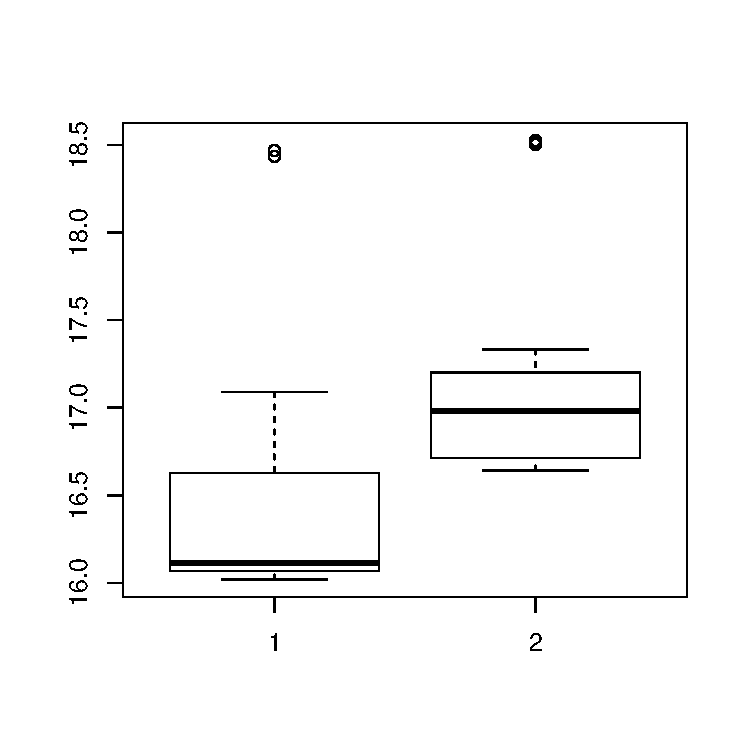
\includegraphics[width=\maxwidth]{figure/r-chunk2-1} 

\end{knitrout}

\subsection{(b)}
I find that the time used to take a subset of these two vectors is nearly same. I do several times comparision, the results are random.
\begin{knitrout}
\definecolor{shadecolor}{rgb}{0.969, 0.969, 0.969}\color{fgcolor}\begin{kframe}
\begin{alltt}
\hlcom{#the function to compare the time used to take a subset of two items.}

\hlstd{compare_subtime}\hlkwb{=}\hlkwa{function}\hlstd{(}\hlkwc{x}\hlstd{,}\hlkwc{y}\hlstd{)\{}
  \hlstd{timex}\hlkwb{=}\hlkwd{microbenchmark}\hlstd{(xsub}\hlkwb{<-}\hlstd{x[}\hlnum{1}\hlopt{:}\hlnum{5}\hlopt{*}\hlnum{1e6}\hlstd{])}\hlopt{$}\hlstd{time}       \hlcom{#get 100 data of time}
  \hlstd{timey}\hlkwb{=}\hlkwd{microbenchmark}\hlstd{(ysub}\hlkwb{<-}\hlstd{y[}\hlnum{1}\hlopt{:}\hlnum{5}\hlopt{*}\hlnum{1e6}\hlstd{])}\hlopt{$}\hlstd{time}
  \hlkwa{if} \hlstd{(}\hlkwd{mean}\hlstd{(timex)}\hlopt{>}\hlkwd{mean}\hlstd{(timey))} \hlkwd{print}\hlstd{(}\hlstr{"taking a subset of the first one takes more time"}\hlstd{)}
  \hlkwa{else} \hlkwd{print}\hlstd{(}\hlstr{'taking a subset of the second one cost more time'}\hlstd{)}
  \hlkwd{boxplot}\hlstd{(}\hlkwd{log}\hlstd{(timex),}\hlkwd{log}\hlstd{(timey))}
\hlstd{\}}


\hlcom{#get the comparation and plot it}
\hlkwd{compare_subtime}\hlstd{(intvec,numvec)}
\end{alltt}
\begin{verbatim}
## [1] "taking a subset of the second one cost more time"
\end{verbatim}
\end{kframe}
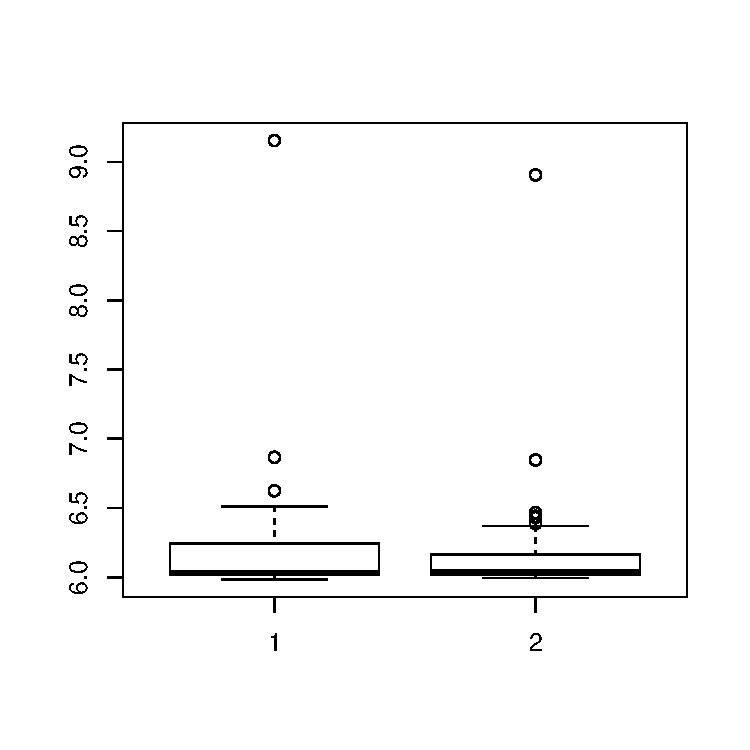
\includegraphics[width=\maxwidth]{figure/r-chunk3-1} 

\end{knitrout}

\section{Question4}
\subsection{(a)}
\quad \ \ Breaking Y into n individual column-wise computations sometimes may not speed up a lot. Because if there is one task needs much more time than any other one, it still takes much time even though we breaking Y into n individual columns. In this way, it can not speed up a lot while it costs much more communication. \\

Therefore sometimes it is better to break up Y into p blocks of m = n/p columns rather than into n individual column-wise computations

\subsection{(b)}
\quad \ \ 1. In approach one, each worker deals with a $\frac{n}{p}\times n$ matrix , plus the memory used to store matrix X, Y. Then the total memory used in a single moment is 
$$\frac{n}{p}\times n\times p+2n^2=3n^2$$ \\

In approach two, each worker deals with a $\frac{n}{p}\times \frac{n}{p}$ matrix , plus the memory used to store matrix X, Y. Then the total memory used in a single moment is 
$$\frac{n}{p}\times \frac{n}{p}\times p+2n^2=2n^2+\frac{n^2}{p}$$ \\

Therefore, the second approach use less memories.\\

2. In approach one, each worker takes in and out numbers only once and it takes in a $n\times \frac{n}{p}$ matrix plus a $n\times n$ matrix, and takes out a $n\times \frac{n}{p}$ matrix. so the total number of numbers needed to be passed is 
$$(2n\times \frac{n}{p}+n\times n)\times p=2n^2+pn^2$$ \\

In approach two, each worker takes in and out numbers p times, it takes in two $\frac{n}{p}\times n$ matrixes and takes out one $\frac{n}{p}\times \frac{n}{p}$ matrix in one time. so the total number of numbers needed to be passed is 
$$(2\times \frac{n}{p}\times n+\frac{n}{p}\times \frac{n}{p})\times p \times p=2pn^2+n^2$$ \\

Therefore, the first approach is better for minimizing the communication.

\section{Question5}


From the question2, we know numerics are written as the following format:
$$(-1)^S*1.d_{1}d_{2}...d_{52}*2^{e-1023}=(-1)^S*(1+d_{1}*2^{-1}+d_{2}*2^{-2}...+d_{52}*2^{-52})*2^{e-1023}$$

I only discuss the situation the number is smaller than 1, without loss of generality. 

It is obviously that only $n=\sum_{i=1}^{52}a_{i}*2^{-i}$can be accurately stored. 

And other numbers are stored as $m=\sum_{i=1}^{52}a_{i}*2^{-i}$, where $a_{i}$ minimizes $\|m-\sum_{i=1}^{52}a_{i}*2^{-i}\|$

Then we take example of 0.2+0.3. If $0.2=\sum_{i=1}^{52}a_{i}*2^{-i}$, $a_{i}$ are fixed there, it shows that $a_{i}$ minimizes
$$\|0.2-\sum_{i=1}^{52}a_{i}*2^{-i}\|$$
And
$$\|0.2-\sum_{i=1}^{52}a_{i}*2^{-i}\|=\|0.3-(2^{-1}-\sum_{i=1}^{52}a_{i}*2^{-i})\|$$
So 0.3 is store as $2^{-1}-\sum_{i=1}^{52}a_{i}*2^{-i}$ in R. Then 0.2+0.3=0.5.

However, if the result can not be written as binary format, like 0.1+0.2=0.3. Then we can not guarantee that it is true.
\begin{knitrout}
\definecolor{shadecolor}{rgb}{0.969, 0.969, 0.969}\color{fgcolor}\begin{kframe}
\begin{alltt}
\hlnum{0.2}\hlopt{+}\hlnum{0.3}\hlopt{==}\hlnum{0.5}
\end{alltt}
\begin{verbatim}
## [1] TRUE
\end{verbatim}
\begin{alltt}
\hlnum{0.1}\hlopt{+}\hlnum{0.4}\hlopt{==}\hlnum{0.5}
\end{alltt}
\begin{verbatim}
## [1] TRUE
\end{verbatim}
\begin{alltt}
\hlnum{0.1}\hlopt{+}\hlnum{0.2}\hlopt{==}\hlnum{0.3}
\end{alltt}
\begin{verbatim}
## [1] FALSE
\end{verbatim}
\end{kframe}
\end{knitrout}


\end{document}
